\scanpage{97}
% archive sheet number: 96
\begin{center}
Filtration et poids des espaces de cohomologie des variétés algébriques

par A.GROTHENDIECK
\end{center}

0. \uline{Introduction}. On a remarqué, depuis \mbox{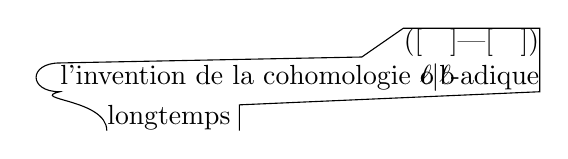
\begin{tikzpicture}[baseline=(old.base)]
\node[inner sep=0] (old) {\deleted{longtemps}};
\node[anchor=south west,inner sep=0,xshift=-1.7em,yshift=1.1ex] (added) at (old.north west) {\inserted{l'invention de la cohomologie $\unsure{\rlap{o}\handwritten{\ell}|\rlap{b}\handwritten{\ell}}$-adiq\handwritten{u\unsure{e}}}};
\node[anchor=south east,inner sep=0,yshift=.5ex] (ref) at (added.north east) {\handwritten{\unsure{([\quad]|[\quad])}}};
\draw (old.south west) .. controls +(0,.4) and +(-.4,-.1) .. (added.south west) .. controls +(-.4,0) and +(-.4,0) .. (added.north west) -- ([xshift=-1.5em]ref.south west) -- (ref.north west) -- (ref.north east) -- (added.south east) -- ([xshift=.3em]old.north east) .. controls +(0,-.1) and +(0,.2) .. ([xshift=.3em]old.south east);
\end{tikzpicture}}, que\deleted{\unsure{x|,}} pour une variété algébrique $X$ définie sur un corps $k$, de clôture algébrique $\bar{k}$, les opérations naturelles du groupe de Galois $\deleted{\unsure{\operatorname{Gal}k|G_k|G(k)}}\handwritten{\pi}=\operatorname{Gal}(\bar{k}/k)$ sur la cohomologie $\handwritten{\ell}$-adique $H(X_{\bar{k}},\underline{Z}_{\handwritten{\ell}})$ de la variété ``géométrique'' $X_{\bar{k}}$ définissait sur cette \mbox{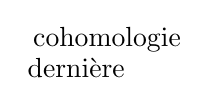
\begin{tikzpicture}[baseline=(old.base)]
\node[inner sep=0] (old) {\deleted{dernière}};
\node[anchor=south west,inner sep=0,xshift=.2em,yshift=.4ex] at (old.north west) {\inserted{\handwritten{cohomologie}}};
\end{tikzpicture}} une structure supplémentaire remarquable, donnant lieu notamment aux remarquables conjectures de Tate \handwritten{[\quad]}. Il semble probable que ces dernières soient n\rlap{\handwritten{e}}\deleted{\unsure{o|e}}t\mbox{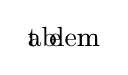
\begin{tikzpicture}[baseline=(old.base)]
\node[inner sep=0] (old) {\deleted{ablem}};
\node[anchor=base west,inner sep=0] at (old.base west) {\handwritten{t}};
\node[anchor=base,inner sep=0,xshift=-.3em] at (old.base) {\handwritten{e}};
\node[anchor=base east,inner sep=0] at (old.base east) {\handwritten{m}};
\end{tikzpicture}}ent plus éloignées d\rlap{\handwritten{e}}\deleted{leur solution} leur solution que les conjectures de Weil \handwritten{[\quad,\quad]}, qui, comme on sait, peuvent s'interpréter également en termes d'actions galoisiennes sur des groupes de cohomologie $\handwritten{\ell}$-adiques. Notre propos dans le présent travail est de montrer comment on peut, des conjectures de Weil et (le cas échéant) de la résolution des singularités, tirer des conséquences de nature ``géométrique'' en apparence, i.e. relatives à un corps de base algébriquement clos. Le principe \mbox{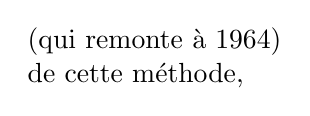
\begin{tikzpicture}[baseline=(base.base)]
\node[inner sep=0] (base) {de cette méthode,};
\node[anchor=south west,inner sep=0,yshift=.6ex] at (base.north west) {\inserted{\deleted{(qui remonte à 1964)}}};
\end{tikzpicture}} qui consiste donc essentiellement à ramener un énoncé géométrique au cas d'un corps de base fini, est expliqué au N\textsuperscript{\uline{o}}1, et des exemples d'application de cette méthode sont donnés dans les numéros 2 à 7. \deleted{Le pr} L'idée de ces raisonnements, liés à\mbox{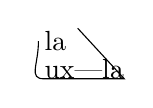
\begin{tikzpicture}[baseline=(old.base)]
\node[inner sep=0] (old) {\deleted{\unsure{ux|la}}};
\node[anchor=south west,inner sep=0,yshift=.6ex] (added) at (old.north west) {\inserted{la}};
\draw ([xshift=-.2em]added.west) .. controls +(0,-.3) and +(-.2,0) .. (old.south west) -- (old.south east) -- ([xshift=.4em,yshift=.1em]added.north east);
\end{tikzpicture}} \mbox{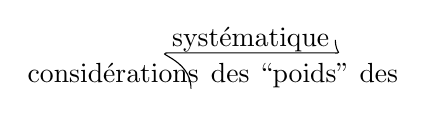
\begin{tikzpicture}[baseline=(base.base)]
\node[inner sep=0] (base) {considération\deleted{\unsure{s}}};
\node[anchor=base west,inner sep=0,xshift=.4em] (right) at (base.base east) {des ``poids'' des};
\node[anchor=south west,inner sep=0,xshift=-1em,yshift=.8ex] (added) at (base.north east) {\inserted{systématique}};
\draw ([xshift=-.3em,yshift=-.5ex]base.south east) .. controls +(0,.4) and +(-.3,0) .. (added.south west) -- (added.south east) .. controls +(.2,0) and +(0,-.2) .. ([xshift=.2em]added.east);
\end{tikzpicture}} modules galoisiens provenant de la cohomologie $\handwritten{\ell}$-adique, remonte à 1964; des exemples \mbox{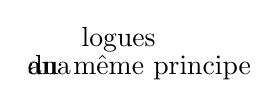
\begin{tikzpicture}[baseline=(du.base)]
\node[inner sep=0] (du) {\deleted{du}};
\node[anchor=base west,inner sep=0,xshift=.5em] (old) at (du.base east) {\deleted{même principe}};
\node[anchor=base west,inner sep=0] at (du.base west) {\handwritten{ana}};
\node[anchor=south west,inner sep=0,xshift=.3em,yshift=.2ex] at (old.north west) {\inserted{\handwritten{logues}}};
\end{tikzpicture}} se trouvent développés dans SGA 7\handwritten{(}I et II\handwritten{)}; dans le séminaire oral\deleted{e} \mbox{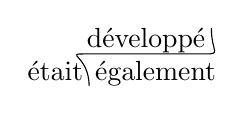
\begin{tikzpicture}[baseline=(left.base)]
\node[inner sep=0] (left) {était};
\node[anchor=base west,inner sep=0,xshift=.4em] (base) at (left.base east) {également};
\node[anchor=south west,inner sep=0,xshift=-.3em,yshift=.6ex] (added) at (base.north west) {\inserted{\handwritten{développé}}};
\draw ([xshift=.2em,yshift=-.4ex]left.south east) .. controls +(0,.4) and +(-.3,0) .. (added.south west) -- (added.south east) .. controls +(.2,0) and +(0,-.3) .. ([xshift=.2em]added.north east);
\end{tikzpicture}} l'exemp\unsure{\rlap{o}l|\rlap{b}l}e du n\textsuperscript{\uline{o}}2 du présent travail.

Bien entendu, la portée des ``résultats'' de notre travail est nécessairement \mbox{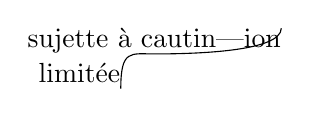
\begin{tikzpicture}[baseline=(old.base)]
\node[inner sep=0] (old) {\deleted{limitée}};
\node[anchor=south west,inner sep=0,xshift=-.4em,yshift=.7ex] (added) at (old.north west) {\inserted{\handwritten{sujette à caut\unsure{in|ion}}}};
\draw ([yshift=-.5ex]old.south east) .. controls +(0,.5) and +(-.3,0) .. (added.south) .. controls +(.5,0) and +(0,-.3) .. (added.north east);
\end{tikzpicture}}, puisqu'ils dépendent de conjectures non prouvées à l'heure actuelle, savoir les conjectures de Weil et la résolution des singularités (sous la forme forte de Hironaka) en caractéristique
